\documentclass[12pt,a4paper]{article}
\usepackage[utf8]{}
\usepackage[T1]{fontenc}


\renewcommand{\baselinestretch}{0.2}

\setlength{\hoffset}{-18pt}         
\setlength{\oddsidemargin}{0pt} % Marge gauche sur pages impaires
\setlength{\evensidemargin}{0pt} % Marge gauche sur pages paires
\setlength{\marginparwidth}{54pt} % Largeur de note dans la marge
\setlength{\textwidth}{481pt} % Largeur de la zone de texte (17cm)
\setlength{\voffset}{-18pt} % Bon pour DOS
\setlength{\marginparsep}{7pt} % Séparation de la marge
\setlength{\topmargin}{0pt} % Pas de marge en haut
\setlength{\headheight}{13pt} % Haut de page
\setlength{\headsep}{4pt} % Entre le haut de page et le texte
\setlength{\footskip}{27pt} % Bas de page + séparation
\setlength{\textheight}{720pt} % Hauteur de la zone de texte (25cm)

\usepackage{natbib}
\usepackage{graphicx}
\usepackage{amssymb}
\usepackage{amsmath} % Required for the align* environment
\usepackage{float}
\usepackage{pgfplots} 
\usepackage{algorithm}
\usepackage{mathrsfs}

\usepackage{algpseudocode} % test comment
\usepackage[hidelinks]{hyperref}
\pgfplotsset{compat=1.18}


\begin{document}
\author{Yunshan Luo}
\title{DD2395 -- Computer security}
\maketitle
\newpage
\section*{Exam analysis}
Do the exam analysis here when needed 

\section{Lecture 2}
\subsection{Alice, Bob, Eve and Mallory}
\begin{itemize}
    \item Alice and Bob tries to send messages to each other
    \item Eve is an eavesdropper, she can read the messages
    \item Mallory is a malicious attacker, she can read and modify the messages
\end{itemize}

\subsection{Three goals fo cryptography}
\begin{itemize}
    \item \textbf{Confidentiality:} Messages cannot be read by anyone except the intended recipient
    \item \textbf{Integrity:} Messages cannot be modified wihtout being detected
    \item \textbf{Authentication:} I can prove that this message came from the person who claims to have sent it
\end{itemize}

\subsection{Keys}
\begin{itemize}
    \item \textbf{Symmetric key:} Alice and Bob both knows the value of the secret key
    \item \textbf{Assymmetric key:} A user has two keys, a secret key and a public key
    \item \textbf{Open design:} Everyone knows how the system is designed
\end{itemize}

\subsection{Confidentiality}
\begin{enumerate}
    \item Alice uses the key to \textbf{encrypt} the message
    \item Alice sends the encrypted message over the insecure channel
    \item Eve sees the encrypted message, but cannot read the original message
    \item Bob receives the encrypted message and uses the key to \textbf{decrypt} the message back into its original form 
\end{enumerate}
\begin{figure}[H]
    \centering
    \includegraphics[width=0.9\textwidth]{Screenshot from 2026-08-31 14-06-04.png}
\end{figure}
\begin{itemize}
    \item \textbf{Plaintext: }The original message
    \item \textbf{Ciphertext: }The encrypted message
\end{itemize}

\subsection{Integrity and Authenticity}
Integrity and authenticity can be provided by using \textbf{tag} or signature on messages
\begin{itemize}
    \item Alice uses the key to generate a tag for the message
    \item Alice sends the message and the tag over the insecure channel
    \item If Mallory modifies the message, Bob will detect it when he checks the tag
    \item Bob receives the message and check if the tag is valid
\end{itemize}
\begin{figure}[H]
    \centering
    \includegraphics[width=0.9\textwidth]{Screenshot from 2026-08-31 14-19-35.png}
\end{figure}

\subsection{Threat models for confidentiality}
\begin{figure}[H]
    \centering
    \includegraphics[width=1\textwidth]{Screenshot from 2026-08-31 14-23-36.png}
\end{figure}
\begin{itemize}
    \item The current lecture focuses on \textbf{Chosen-plaintext} 
\end{itemize}

\subsection{Cryptography Roadmap}
\begin{itemize}
    \item Symmetric-key
    \begin{itemize}
        \item Confidentiality:
        \begin{itemize}
            \item One-time pad
            \item Block ciphers (e.g. AES)
        \end{itemize}
        \item Integrity and authenticity:
        \begin{itemize}
            \item Hash functions
            \item MACs (e.g. HMAC) - Message Authentication Code
        \end{itemize}
    \end{itemize}
        \item Assymmetric-key
        \begin{itemize}
            \item Confidentiality:
            \begin{itemize}
                \item RSA encryption
                \item ElGamal encryption
            \end{itemize}
            \item Integrity and authenticity:
            \begin{itemize}
                \item Digital signatures (e.g. RSA, ECDSA)
            \end{itemize}
    \end{itemize}
\end{itemize}

\subsection{Symmetric Key Cryptography}
Alice and Bob shares a secret key. Symmetric cryptography has three algorithms:
\begin{enumerate}
    \item KeyGen() $\rightarrow$ Generates a key $K$
    \item Enc($K$, $M$) $\rightarrow$ Encrypts \textbf{plaintext} $M$ into \textbf{ciphertext} $C$
    \item Dec($K$, $C$) $\rightarrow$ Decrypts \textbf{ciphertext} $C$ using the key $K$
\end{enumerate}

\subsection{Confidentiality: IND-CPA definition}
\begin{enumerate}
    \item Eve may choose plaintext to send to Alice and receives their chiphertexts
    \item Eve issues a pair of plaintexts $M_0$ and $M_1$ to Alice
    \item Alice chooses either $M_0$ or $M_1$ encrypts it and do not tell Eve which one she chose
    \item Eve may again choose plaintext to send to Alice and receives their ciphertexts
    \item Eve guesses which plaintext Alice chose and wins if she guesses correctly
\end{enumerate}
An algorithm is \textbf{IND-CPA} secure if Eve cannot guess with probability larger than $50\% + \epsilon$. Where $\epsilon$ is a negligible advantage.

\subsection{Edge case: Length}
\begin{itemize}
    \item Cryptographic schemes are not allwed to leak the length of the message
    \item To prevent this there are two solutions:
    \begin{itemize}
        \item Make all messages the same length (unpractical)
        \item Pad messages to a fixed length (practical)
    \end{itemize}
\end{itemize}

\subsection{Negligible advantage}
For an encryption scheme with a k-bit key the advantage for Eve should be $\mathcal{O}(1/2^k)$.
\begin{itemize}
    \item $\epsilon = (\frac{1}{2})^{128}$ -- Currently unlikely
    \item $\epsilon = (\frac{1}{2})^{20}$ -- Fairly likely
    \item \textbf{Takeaway:} $\epsilon < (\frac{1}{2})^{80}$ is a current reasonable threshold
\end{itemize}

\subsection{One-Time pad key generation}
\noindent Encryption scheme
\begin{itemize}
    \item Given a random key $K$ of length $n$
    \item Given a message $M$ of length $n$
    \item $C = M \oplus K$ where $\oplus$ is the bitwise XOR operation
\end{itemize}

\noindent Decryption scheme
\begin{itemize}
    \item Given a random key $K$ of length $n$
    \item Given a ciphertext $C$ of length $n$
    \item $M = C \oplus K$ where $\oplus$ is the bitwise XOR operation
\end{itemize}

\subsection{One-Time pad functions}
\begin{itemize}
    \item \textbf{KeyGen()}
    \begin{itemize}
        \item Randomly generate an n-bit key $K$, where n is the length of your message
        \item We assume that Alice and Bob have a secure channel to share the key
        \item We generate a new key for every message
    \end{itemize}
    \item \textbf{Enc(K, M)}
    \begin{itemize}
        \item $M \oplus K = C$
    \end{itemize}
    \item \textbf{Dec(K, C)}
    \begin{itemize}
        \item $C \oplus K = M$
    \end{itemize}
\end{itemize}

\noindent One-Time pad is \textbf{perfectly secure} however not IND-CPA secure since the key can only be used once.

\section{Lecture 3}
\subsection{Block cipher}
\begin{itemize}
    \item An algorith that encrypts a fixed-size block of bits
    \item $E(K,M) = C$: Encryption
    \begin{itemize}
        \item Inputs: k-bit key $K$ and n-bit plaintext $M$
        \item Output: n-bit ciphertext $C$
        \item Written as $\{0,1\}^k \times \{0,1\}^n \rightarrow \{0,1\}^n$
    \end{itemize}
    \item $D(K,C) = M$: Decryption
    \begin{itemize}
        \item Inputs: k-bit key $K$ and n-bit ciphertext $C$
        \item Output: n-bit plaintext $M$
        \item Written as $\{0,1\}^k \times \{0,1\}^n \rightarrow \{0,1\}^n$
    \end{itemize}
    \item Properties of block ciphers
    \begin{itemize}
        \item $E_k$ is a permutation, $D_k$ is the inverse permutation
        \item Encryption and decryption is fast
        \item $E$ behaves like a random permutation
        \item $E(K,M)$ is always bijective 
    \end{itemize}
\end{itemize}

\subsection{Block cipher: Brute force attacks}
How hard is brute forcing a 128-bit key?
\begin{enumerate}
    \item We have to try $2^{128}$ keys
    \item $2^10 \approx 10^3$
    \begin{itemize}
        \item $2^{128} = (2^{10})^{12.8} \approx (10^3)^{13} = 10^{39}$ 
    \end{itemize}
    \item Supposed that we could try $10^{18}$ keys per second
    \item $10^{39} / 10^{18} = 10^{21}$ seconds $\approx$ 30 trillion years
\end{enumerate}
\newpage
\subsection{AES algorithm}
\begin{enumerate}
    \item Take plain text and shuffle it using the key
    \item Key sizes determines the rounds of shuffling
    \begin{itemize}
        \item 128-bit key: 10 rounds
        \item 192-bit key: 12 rounds
        \item 256-bit key: 14 rounds
    \end{itemize}
    \item Each round uses its own "round key" derived from the cipher key
    \item Each round consists of four operations:
    \begin{enumerate}
        \item \textbf{SubBytes()}: Each byte is replaced with a corresponding byte from a fixed table
        \item \textbf{ShiftRows()}: Each row of the state is shifted by a certain number of bytes
        \item \textbf{MixColumns()}: Each column of the state is multiplied by a fixed polynomial
        \item \textbf{AddRoundKey()}: Each byte of the state is XORed with a byte of the round key
    \end{enumerate}
\end{enumerate}
\begin{figure}[H]
    \centering
    \includegraphics[width=0.65\textwidth]{AES.png}
\end{figure}

\subsection{IND-CPA analysis of block ciphers}
\begin{enumerate}
    \item Eve sends a pair of plaintexts $M_0$ and $M_1$ to Alice
    \item Eve receives the ciphertext $C$ of either $M_0$ or $M_1$ from Alice
    \item Eve requests the encryption of M0 again and receives the ciphertext $C_0$ from Alice
    \item \textbf{Strategy:} If $C = C_0$, then Eve guesses that Alice encrypted $M_0$, otherwise she guesses that Alice encrypted $M_1$
    \item Eve is guaranteed to guess correctly. Therefore not IND-CPA secure
\end{enumerate}

\subsection{Pros and cons of block ciphers}
\begin{itemize}
    \item Block ciphers are not IND-CPA secure
    \begin{itemize}
        \item The algorithm is \textbf{deterministic} because the same input always produces the same output
        \item A determinstic algorithm can never be IND-CPA secure because Eve can always guess correctly by sending the same plaintext twice
    \end{itemize}
    \item Block ciphers can only encrypt messages of a fixed size e.g. only 128 bits for AES
    \item Block ciphers uses XORs and bitshiting which is very fast and efficient
\end{itemize}

\subsection{Crypotgraphic Hashes}
Hash function $H(M)$ properies:
\begin{itemize}
    \item \textbf{Input:} Arbitrary length message $M$
    \item \textbf{Output:} Fixed length hash $h$
    \item \textbf{Deterministic:} The same input always produces the same output
    \item \textbf{Efficient:} The hash can be computed quickly
    \item \textbf{Security properties:} One way (preimage resistant), Collision resistance, random oracle
    \begin{itemize}
        \item \textbf{Random oracle:} There's no way to predict how changing the input will change the output
    \end{itemize}
\end{itemize}

\subsection{Preimage resistance}
\begin{itemize}
    \item \textbf{Informal definition:} Given an input $y$, it's infeasible to find any input $x$, such that $H(x) = y$
    \item \textbf{Formal definition: } $\forall A \in \mathcal{O}(n^k), \hspace{10pt} \Pr[A(H(x)) = y] < \epsilon, \hspace{10pt} \epsilon \approx 0$
\end{itemize}

\subsection{Collision resistance}
Collision is when two different inputs results in the same output
\begin{itemize}
    \item \textbf{Definition} $\forall x \neq x', \hspace{10pt} H(x) \neq H(x')$
    \item Hash functions ith no collisions are impossible due to the pigeonhole principle
    \begin{itemize}
        \item \textbf{Pigeonhole principle:} If you have more pigeons than pigeonholes, at least one pigeonhole must contain more than one pigeon
        \item In this case there are more possible inputs than outputs, so at least two inputs must map to the same output
    \end{itemize}
\end{itemize}

\subsection{Second preimage resistance}
\begin{itemize}
    \item \textbf{Definition:} Given an input $x$, it's infeasible to find another input $x' \neq x$, such that $H(x) = H(x')$
    \item Strong collision resistance $\implies$ Second preimage resistance
    \item \textbf{Collision resistance: } Attacker tries to find two inputs such that $H(x) = H(x')$
    \item \textbf{Second preimage resistance: } Attacker is any given an input $x$ and tries to find another input $x' \neq x$ such that $H(x) = H(x')$
    \item Broken second preimage resistance $\implies$ Broken collision resistance
\end{itemize}

\subsection{Length extension attacks}
\begin{itemize}
    \item \textbf{Length extension attack:} Given $H(x)$ and the length of $x$, but not x, an attacker can create $H(x || m)$ for any $m$ without knowing $x$
    \item SHA-1 and SHA-2 are vulnerable to length extension attacks
    \item SHA-3 is not vulnerable to length extension attacks
\end{itemize}

\subsection{Hashing and integrity}
\begin{itemize}
    \item Hashes themselves are unkeyed functions and don't provide integrity or authenticity
    \item Hashes can be used to build keyed functions that provide integrity and authenticity
\end{itemize}

\subsection{Message Authentication Codes (MACs)}
\begin{enumerate}
    \item Alice wants to send $M$ to Bob, but doesn't want Mallory to tamper with it 
    \item Alice sends $M$ and $T = MAC(K, M)$ to Bob
    \item Bob recomputes $MAC(K, M)$ and checks if it equals $T$
    \item If $MAC(K, M) = T$, Bobs'is confident that the message has not been tampered with
\end{enumerate}
\begin{figure}[H]
    \centering
    \includegraphics[width=0.9\textwidth]{mac.png}    
\end{figure}

\subsection{MACs: Definition}
MACs consists of two parts:
\begin{enumerate}
    \item $KeyGen() \rightarrow K$: Generates a key $K$
    \item $MAC(K, M) \rightarrow T$: Generates a tag $T$ for $M$ using $K$
\end{enumerate}

The three properties of MACs are:
\begin{enumerate}
    \item \textbf{Correctness: }Determinism 
    \item \textbf{Efficiency: }Computing MAC should be efficient 
    \item \textbf{Security: }EU-CPA i.e existentially unforgeable under chosen plaintext attack
\end{enumerate}

\subsection{EU-CPA definition}
\begin{itemize}
    \item A secure MAC is \textbf{existentially unforgeable: }without the key, an attacker cannot create a valid tag on a message
    \begin{itemize}
        \item Mallory cannot find $M' \neq M$ such that $MAC(K, M') = MAC(K, M)$
    \end{itemize}
    \item MACs should be unforgeable under chose plaintext attack
    \begin{itemize}
        \item Even if Mallory can trick Alice into creating MACs for messages of Mallory's choosing, Mallory cannot create a valid MAX on a message that she hasn't seen before
    \end{itemize}
\end{itemize}

\subsection{EU-CPA game}
\begin{enumerate}
    \item Mallory may send messsages to Alice and receive their tags
    \item Eventually, Mallor creates a message-tag pair (M', T')
    \begin{itemize}
        \item M' cannot be the message that mallory requested earlier
        \item If T' is a valid tag for M', then Mallory wins
    \end{itemize}
    \item A scheme is EU-CPA secure if Mallory cannot win in polynomial time with probability larger than $\epsilon$, where $\epsilon$ is negligible
\end{enumerate}

\begin{figure}[H]
    \centering
    \includegraphics[width=0.5\textwidth]{eucpa.png}
\end{figure}

\subsection{NMAC}
\begin{itemize}
    \item Using cryptographic hash functions to build secure MACs
    \item $KeyGen()$: Outputs two random, n-bit $K_1$ and $K_2$, where $n$ is the length of the hash output
    \item \textbf{NMAC}: $NMAC(K_1, K_2, M)$: outputs $H(K_2 || H(K_1 || M))$, where $||$ is concatenation
    \item \textbf{Security}: NMAX is EU-CPA secure if the two keys are different 
    \item By using two hashes with different keys, we prevent length extension attacks
    \item Issues with NMAC:
    \begin{itemize}
        \item Two keys are needed
        \item NMAC requires the keys to be the same length as the hash output
    \end{itemize}
\end{itemize}

\subsection{HMAC}
$HMAC(K, M)$:
\begin{itemize}
    \item Compute $K'$ as a version of $K$ that is the length of the hash output
    \item If K is too short, pad $K$ with 0's to make it $n$ bits (Be careful with $K$ that are too short due to lack of randomness)
    \item If K is too long, hash $K$ to make it $n$ bits
    \item Output $H(K' \oplus opad || H(K' \oplus ipad || M))$, where $opad$ and $ipad$ are fixed constants
\end{itemize}

\noindent Use $K'$ to derive two different kyes
\begin{itemize}
    \item oad (outer pad): hard-coded constant byte 0x5c repeated until the length of the hash output
    \item ipad (inner pad): hard-coded constant byte 0x36 repeated until the length of the hash output
    \item As long as \textbf{opad} and \textbf{ipad} are different, you'll get two different keys
\end{itemize}

\noindent HMAC properties:
\begin{itemize}
    \item $HMAC(K,M) = H(K' \oplus opad || H(K' \oplus ipad || M))$
    \item $HMAC$ is a hash function, so it has the properties of the underlying hash 
    \item You can't verify a tag $T$ if you don't have $K$
\end{itemize}

The three cryptographic questions regarding HMAC are:
\begin{enumerate}
    \item Integrity
    \begin{itemize}
        \item Mallory cannot tamper with the message without being detected
    \end{itemize}
    \item Authenticity
    \begin{itemize}
        \item If two people share a secret key, they can be sure that the message came from the other person
    \end{itemize}
    \item Confidentiality
    \begin{itemize}
        \item MACs are deterministic $\implies$ no IND-CPA security 
        \item MACs in general have no confidentiality guarantees, they can leak information about the message
    \end{itemize}
\end{enumerate}

\subsection{Authenticated Encryption (AE)}
\begin{itemize}
    \item \textbf{Authenticated encryption (AE):} A scheme that simultaneously guarantees confidentiality and integrity
    \item The two main approaches to AE are:
    \begin{enumerate}
        \item Combine schemes that provide confidentiality with schemes that provide integrity
        \item Use a scheme that is designed to provide both confidentiality and integrity (not in the course)
    \end{enumerate}
\end{itemize}

\subsection{MAC-then-Encrypt or Encrypt-then-MAC?}
Mac-then-encrypt
\begin{itemize}
    \item First compute $MAC(K_2, M)$ 
    \item Then encrypt message and the MAC together: $Enc(K_1, M || MAX(K_2, M))$
    \item Both are IND-CPA and EU-CPA secure 
    \begin{itemize}
        \item However, for MAC-then-encrypt you don't know if tampering has occured until after decrypting
        \item Therefore, Encrypt-then-MAC is preferred
    \end{itemize}
\end{itemize}

\subsection{Digital signatures}
\begin{itemize}
    \item Asymmetric cryptography means that we don't need to share a secret key
    \item Digital signatures are the asymmetric way of providing integrity/authenticity
    \item Assume that Alice and Bob can communicate public keys without Mallory changing them
    \item The owner can sign message with their private key that anyone can verify with their public key
\end{itemize}

\subsection{Digital signatures: Definition}
\begin{itemize}
    \item Three parts
    \begin{itemize}
        \item $KeyGen() \rightarrow PK, SK$: Generates a public/private keypair, where PK is the verify key and SK is the sign key
        \item $Sign(SK,M) \rightarrow sig$: Sign the message M using the signing key SK to produce the signature sig
        \item $Verify(PK, M, sig) \rightarrow \{0,1\}$: Verify the signature sig on the message M using the verify key PK. Returns 1 if valid, 0 otherwise
    \end{itemize}
    \item Properties
    \begin{enumerate}
        \item \textbf{Correctness}: Verification should be successful for a signature generated over any message
        \begin{itemize}
            \item $Verify(PK, M, Sign(SK, M)) = 1, \hspace{10pt} \forall PK, SK \leftarrow KeyGen()$ and $M$
            \item \textbf{Efficiency: }Signing and verifying should be fast
            \item \textbf{Security: }EU-CPA, same as for MACs
        \end{itemize}
    \end{enumerate}
\end{itemize}

\subsection{Digital signatures in practice}
\begin{itemize}
    \item If you want to sign a message $M$:
    \begin{enumerate}
        \item Hash $M$
        \item Then $Sign(SK, H(M))$ to produce the signature signature
    \end{enumerate}
    \item We use hash to allow arbitrarily long messages
    \item Digital signatures provide integrity and authenticity
\end{itemize}

\section{Lecture 4}
\begin{itemize}
    \item \textbf{Authentication:} Mechanisms that bind principals to actions
    \item \textbf{Authorization:} Mechanisms that govern wwhether actions are permitted
    \item \textbf{Audit:} Mechanisms that record and review actions (not included in this course)
\end{itemize}

\subsection{Authentication}
Mechanisms that bind principals to actions
\begin{itemize}
    \item Authenticating humans
    \item Authenticating machines
\end{itemize}
\begin{figure}[H]
    \centering
    \includegraphics[width=0.9\textwidth]{Authentication.png}
\end{figure}

\subsection{Identity}
\begin{itemize}
    \item \textbf{Attribute:} Property of a principal (e.g. age, gender, height)
    \item \textbf{Identity:} A principal may have many identities of use in different scenarios (e.g. work, home, school)
    \item \textbf{Identifier:} An attribute that uniquely identifies a principal within a given context (e.g. username, email address)
    \item \textbf{Authentication:} Check if an identity matches a set of attributes
    \begin{itemize}
        \item \textbf{Example:} ICE checks if a person is who they say on their passport
    \end{itemize}
\end{itemize}

\subsection{Identity enrollement}
\begin{itemize}
    \item \textbf{Enrollment:} Establishing identity with a system
    \begin{itemize}
        \item Create an account 
        \item Get an ID card or visa
        \item Register a machine with a network
        \item Get a signing key from a provider
    \end{itemize}
\end{itemize}

\subsection{Authentication of humans to machines}
\begin{itemize}
    \item Something you are
    \begin{itemize}
        \item Biometrics: Fingerprint, iris scan, face recognition
    \end{itemize}
    \item Something you know
    \begin{itemize}
        \item Password, PIN, secret question
    \end{itemize}
    \item Something you have
    \begin{itemize}
        \item Physical token, smart card, phone
    \end{itemize}
\end{itemize}

\subsection{Authentication of humans to machine}
\begin{itemize}
    \item Two-factor authentication (2FA)
    \begin{itemize}
        \item ATM card + PIN
        \item Password + SMS code
    \end{itemize}
    \item Multi-factor authentication (MFA)
    \begin{itemize}
        \item Two or more independent methods of authentication
    \end{itemize}
\end{itemize}

\subsection{Passwords}
All these steps are tricky and subject to compromise
\begin{enumerate}
    \item \textbf{Create:} Users chooses password
    \item \textbf{Store:} System stores password
    \item \textbf{Use:} User supplies password to authenticate
    \item \textbf{Change/recover/reset:} User wants or needs to change password
\end{enumerate}

\subsection{Weak passwords}
\begin{itemize}
    \item Users often choose weak passwords that are easy to remember
    \item The top 20 most common passwords in 2024 are enough to compromise 10\% of accounts 
\end{itemize}

\subsection{Strong passwords}
\begin{itemize}
    \item Difficult to breute force or guess
    \begin{itemize}
        \item $2^X$ guesses required, strength is $X$
    \end{itemize}
    \item Assume passwords are $L$ characters long and each character is chosen from a set of $N$ characters
    \item \begin{itemize}
        \item Then $N^L$ guesses are required to brute force the password
        \item Strength of the password is $X = L \log_2(N)$
    \end{itemize}
    \item $X$ is known as the \textbf{entropy} of the password
    \item Shannon entropy states that every passwords is equally likely which is not entirely true
\end{itemize}

\subsection{Entropy of passwords}
Example A:
\begin{enumerate}
    \item 8 character password chosen uniformly at random from 26 character alphabet
    \item Entropy of $8\log_2(26) \approx 37$ bits
    \item Assuming that abcdefgh is just as likely inaopas which is not true
\end{enumerate}

\noindent Example B:
\begin{itemize}
    \item 1 word chosen at random from entire vocabulary of 50k words
    \item Entropy of $\log_2(50000) \approx 16$ bits
\end{itemize}

\noindent \textbf{Problem:} Shannon enropy not a good measure of how secure a password is

\subsection{Password storage and usage}
\begin{itemize}
    \item \textbf{Password:} A secret string that the user types to prove their identity
    \begin{enumerate}
        \item \textbf{Account creation:} User creates a passowrd 
        \item \textbf{Log in:} User types password to prove identity
    \end{enumerate}
\end{itemize}
\noindent How to store password securely?
\begin{itemize}
    \item \textbf{Bad idea 1:} Store a file with the password in plaintext
    \item \textbf{Bad idea 2:} Encrypt the password with a key and store the ciphertext
\end{itemize}
\noindent We need a way to store passwords that allows us verify without storing information that allows someone to easily get the original password

\subsection{Password hashing}
Define a function $f$ such that 
\begin{enumerate}
    \item Easy to compute and store $f(p)$ for a password $p$
    \item Hard to compute $f^{-1}(f(p))$ to get $p$ from $f(p)$
    \item Hard to trick the system by finding $q \neq p$ such that $f(q) = f(p)$
\end{enumerate}

\noindent \textbf{Cryptographic hash those properties by:}
\begin{itemize}
    \item One-wayness: Hard to compute $f^{-1}(f(p))$ to get $p$ from $f(p)$
    \item Collision resistance: Hard to find $q \neq p$ such that $f(q) = f(p)$
\end{itemize}

\noindent The secure process is:
\begin{itemize}
    \item Store the hash of user passwords 
    \item Hash the password submitted by user and compare it to the stored hash
    \item If they match, the user is authenticated
\end{itemize}

\subsection{Authentication process}
Each user has:
\begin{itemize}
    \item \textbf{Username:} $uid$
    \item \textbf{Password:} $p$
\end{itemize}

\noindent The system stores:
\begin{itemize}
    \item \textbf{Username:} $uid$
    \item \textbf{Password hash:} $h = H(p)$
\end{itemize}

\subsection{Password hashing attacks}
\begin{itemize}
    \item Hashes are deterministic 
    \item If two users have the same password they'll have the same hash
\end{itemize}

\noindent Brute force attacks:
\begin{itemize}
    \item \textbf{Dictionary attack:} Hash an entire dictionary of common passwords
    \item It works because passwords chosen by human are from a relatively small set
    \item \textbf{Rainbow tables:} An algorithm for computing hashes that makes brute force attacks faster by storing precomputed hashes of common passwords
\end{itemize}

\subsection{Salted hashed passwords}
Each user has:
\begin{itemize}
    \item username $uid$
    \item password $p$
    \item unique salt $s$ 
\end{itemize}
\noindent System stores: $uid, s, H(s, p)$
\begin{verbatim}
    // When a user logs in:
    let h = stored hashed password for uid
    let s = stored salt for uid
    if H(s, p) == h:
        authentication successful
    else:
        authentication failed
\end{verbatim}
\begin{itemize}
    \item The users salts are not secret but they are unique and random
\end{itemize}

\subsection{How salt makes brute forcing harder?}
\begin{itemize}
    \item Suppose there are $M$ possible passwords and $N$ users in the database
    \item Un-salted hashes: The attacker can compute $M$ hashes and check them against all $N$ users, $O(M+N)$
    \item Salted hash: Attacker must hash all passwords for each user salt, $O(MN)$
    \item Furthermore if one user has a unique salt, the attacker cannot use precomputed rainbow tables
\end{itemize}

\subsection{Defense against Online Attack}
\begin{itemize}
    \item Don't leak valid usernames
    \begin{itemize}
        \item Prompt for username and password together
        \item Don't tell which one is wrong
    \end{itemize}
    \item Rate limit login attempts
    \item Lock account after certain number of failed attempts
\end{itemize}

%% Sida 28 föreläsning 4

\subsection{Rate limiting}
\begin{itemize}
    \item Cryptographic hashes are generally designed to be fast to compute  
    \item By slowing down hashes to barely affects login speed but signficantly slows down brute force attacks
    \item Such hashes are called password hashes which are designed to be slow
\end{itemize}

\subsection{How to slow down a fast hash}
\begin{itemize}
    \item Given a fast hash $H$
    \item We can slow it down by computing $H$ multiple times
    \item For example:
    \begin{enumerate}
        \item $z_1 = H(p)$
        \item $z_2 = H(p, z_1)$
        \item $z_3 = H(p, z_2)$
        \item $\vdots$
        \item $z_k = H(p, z_{k-1})$
    \end{enumerate}
    \item The number of iterations can be chosen arbitarily 
\end{itemize}

\subsection{Slow hashes: PBKDF2}
\textbf{Password-based key derivation function 2}
\begin{itemize}
    \item \textbf{Settings}
    \begin{enumerate}
        \item An underlying function that outputs random-looking bits (e.g. HMAC-SHA256)
        \item The desired length of the output $n$
        \item Iteration count $c$ (e.g. 100k)
    \end{enumerate}
    \item \textbf{Inputs}
    \begin{enumerate}
        \item Password $p$
        \item Salt $s$
    \end{enumerate}
    \item \textbf{Output:} n-bit string derived rom $p$ and $s$
    \item \textbf{Benefits:}
    \begin{enumerate}
        \item Derives an abitrarily long string from the user's password
        \item Output can be used as a key for symmetric encryption
        \item Algorithm is slow without hogging memory
    \end{enumerate}
\end{itemize}

\subsection{Authorization}
\begin{itemize}
    \item \textbf{Authentication:} Mechanisms that binds principals to actions
    \item \textbf{Authorization:} Mechanisms that govern whether actions are permitted
\end{itemize}

\subsection{Access control policy}
An \textbf{acess control policy} specifies which of the \textbf{operations} associated with any given \textbf{object} each principal is auhtorized to perform.
\begin{figure}[H]
    \centering
    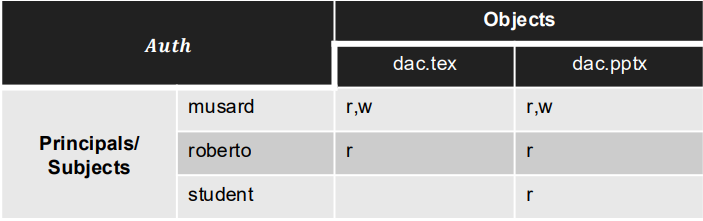
\includegraphics[width=0.75\textwidth]{access.png}
\end{figure}

\subsection{Access control mechanisms}
\begin{itemize}
    \item A \textbf{reference monitor} is consulted whenever one of a predefined set operation is invoked
    \item Can enforce confidentiality and integrity 
\end{itemize}

\subsection{Discretionary and mandatory access control}
\begin{itemize}
    \item \textbf{Discretionary access control (DAC):} The owner of an object can determine who is authorized to access it
    \item \textbf{Mandatory access control (MAC):} Centralized authority determines authorizations 
\end{itemize}

\subsection{Discretionary Access Control (DAC)}
\textbf{Design principles: }
\begin{itemize}
    \item \textbf{Principle of Failsafe Defaults:} Defning an access control policy by enumerating privleges rather than prohibitions
    \item \textbf{Principle of Least Privilege:} Every program and every user of the system should operate using the least set of privileges necessary to complete the job
\end{itemize}
\textbf{Protection domains:}
\begin{itemize}
    \item Each thread of control is associated with a protection domain
    \item Each protection domain is associated with a different set of priveleges
    \item We allow transitions from one protection domain to another as execution of the thread proceeds
\end{itemize}
\textbf{Protection domains transitions:}
\begin{itemize}
    \item \textbf{Attenuation of priviledge:} Transition into a protected domain that eliminates privileges
    \item \textbf{Amplification of privelege:} Transition into a protected domain that adds privileges
\end{itemize}
\begin{figure}[H]
    \centering
    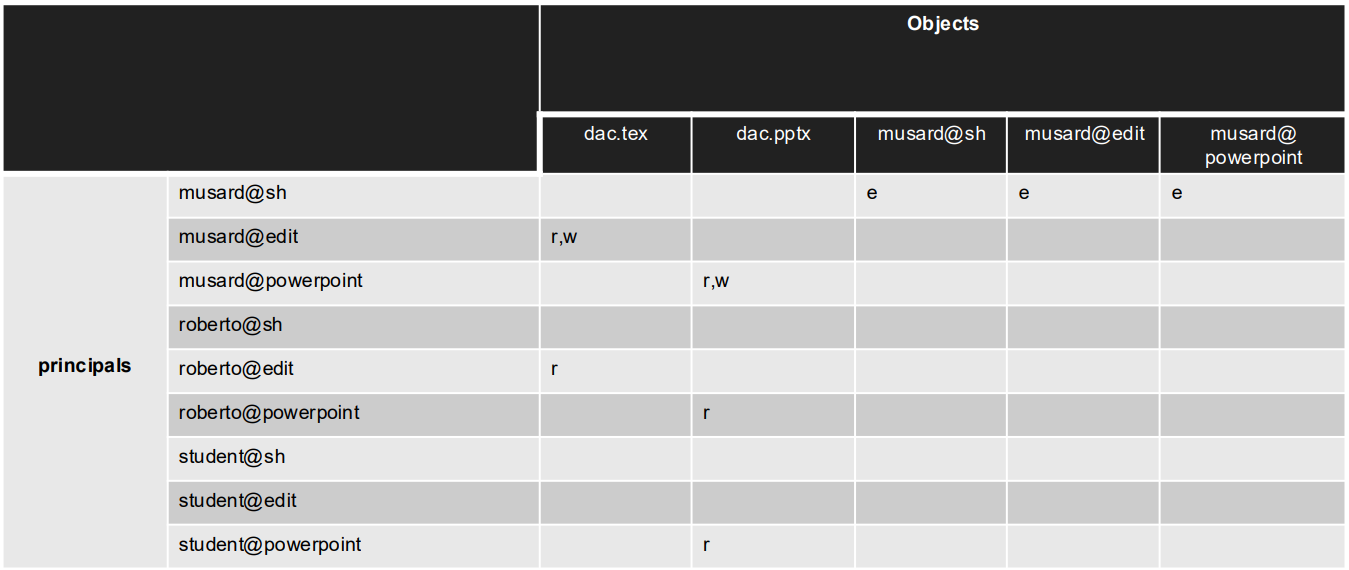
\includegraphics[width=1\textwidth]{protection.png}
\end{figure}

\subsection{Implementing DAC}
\begin{itemize}
    \item $P$ is a principal
    \item $O$ is an object
    \item $op$ is an operation
\end{itemize}

We need to compute $<P, O, op> \in Auth$ 
\begin{itemize}
    \item Instead of illustrating this in a matrix access control lists are used instead
\end{itemize}

Example of an access control list:
\begin{verbatim}
    <musard, {r,w}>
    <alice, {r}>
    <student, {r}>
\end{verbatim}

\noindent \textbf{Adantages and disadvantages}
Advantages:
\begin{itemize}
    \item Efficient review of permission for given object
    \item Centralized enforcement is simply to deploy and verify 
    \item Revocation is straightforward
\end{itemize}
Disadvantages:
\begin{itemize}
    \item Inefficient review of permission for given principal
    \item Large lists impede performance
    \item Vulnerable to confused deputy attacks
\end{itemize}

\subsection{Confused deputy}
Assume a service that has these 5 steps:
\begin{enumerate}
    \item \textbf{Buffer} $\leftarrow$ FileSys.Read(f)
    \item \textbf{Results} $\leftarrow$ function(buffer)
    \item \textbf{chrgs} $\leftarrow$ calcBill(results)
    \item \textbf{FileSys.Write(f, results)}
    \item \textbf{FileSys.Write(changes, chrgs)}
\end{enumerate}
In step 4 if we switch the file $f$ to a different file, the service will write to that file instead of the intended one. The service is confused into writing to a file that it should not have access to.

\subsection{Solution: Confused deputy}
\begin{enumerate}
    \item Combining nameing with authorization: Don't allow write to a file it doesn't have access 
    \item Replace names with unforgable bundles i.e object name + privledges
    \item Client conveys a bundle for file $f$ which server uses to read and update $f$
    \item Server already has a bundle for charges.txt
    \item Client supplied bundle for charges.txt does not have write privlege 
\end{enumerate}

\subsection{Capability lists}
A capability list for a principal $P$ can look liek
\begin{verbatim}
    <doc1, {r,w}>
    <doc2, {r}>
    <doc3, {r}>
\end{verbatim}

\begin{itemize}
    \item To perform operation $op$ on object $O$, the system checks if $<O, op> \in Cap(P)$
\end{itemize}

\subsection{C-lists}
\begin{itemize}
    \item The OS stores list of capabilities $C_i = <O_i, Privs_i>$ for each principal $P_i$
\end{itemize}
\begin{enumerate}
    \item \textbf{Authorization:} OS mediates access to objects, checks process capabilities
    \item \textbf{Unforgeability:} Capabilities are stored in protected memory region (kernel memory)
\end{enumerate}

\begin{figure}[H]
    \centering
    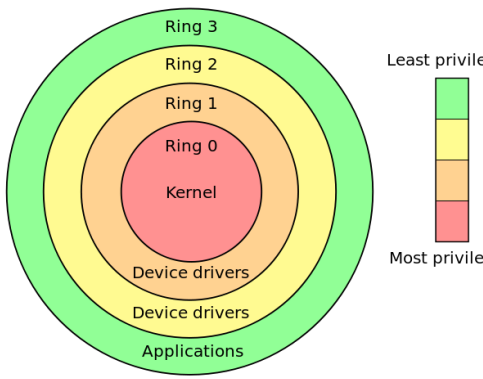
\includegraphics[width=0.5\textwidth]{kernel.png}
\end{figure}

\subsection{Summary DAC}
Discretionary access control (DAC) 
\begin{itemize}
    \item \textbf{Philosophy:} Users have the discretion to specify policies themselves
    \item Access control authorization \textbf{relation}
    \begin{itemize}
        \item Set of triplets (subject, object, rights)
        \item Described as access control "matrix"
    \end{itemize}
\end{itemize}

Implementations:
\begin{itemize}
    \item \textbf{Access control lists (ACLs):} Each object associated with list of (subject, rights)
    \item \textbf{Capability lists (Privilege lists):} Each subject associated with list of (object, rights)
\end{itemize}

\subsection{Multi-level security}
Principals and objects are assigned security levels
\begin{enumerate}
    \item Verified protection: Top secret
    \item Mandatory protection: Secret
    \item Discretionary protection: Confidential
    \item Unclassified: Minimal protection  
\end{enumerate}
\begin{itemize}
    \item \textbf{Need to know principle:} Access should be granted only when necessary to perform assigned duties
\end{itemize}
Access control policy 
\begin{itemize}
    \item Subject may read an object only if the subject's security level is greater than or equal to the object's security level
    \item Subject may write to an object only if the subject's security level is less than or equal to the object's security level
    \item Subject must be within the objects label to read or write to it
\end{itemize}

\subsection{Writing with MLS}
\begin{itemize}
    \item \textbf{Blind write:} Subject may not read high security object yet may write ti 
    \item \textbf{Trojan horse prevention:} Subject may not write lower security object yet may read it
\end{itemize}

\section{Cryptography}
Mode of operation for block ciphers:
\begin{itemize}
    \item \textbf{Electronic Codebook (ECB):} Each block is encrypted independently
    \item \textbf{Cipher Block Chaining (CBC):} Each block is XORed with the previous block's ciphertext
    \item \textbf{Counter (CTR):} Each block is XORed with a counter
\end{itemize}
\begin{itemize}
    \item \textbf{Assymmetric cyrptography:} 
    \begin{itemize}
        \item Diffie-Hellman key exchange
        \item RSA
    \end{itemize}
\end{itemize}

\subsection{Block ciphers}
\begin{itemize}
    \item \textbf{Encryption:} 
    \begin{itemize}
        \item \textbf{Input:} $k$-bit key $K$ and $n$-bit plaintext $P$
        \item \textbf{Output:} $n$-bit ciphertext $C$
    \end{itemize}
    \item \textbf{Decryption:}
    \begin{itemize}
        \item \textbf{Input:} $k$-bit key $K$ and $n$-bit ciphertext $C$
        \item \textbf{Output:} $n$-bit plaintext $P$
    \end{itemize}
    \item $E(K,M)$ should be bijective and efficient
\end{itemize}

\subsection{ECB mode of operation}
How to encrypt message of arbitrary length using AES, given a key and that stanard AES only encrypts 128-bit blocks:
\begin{enumerate}
    \item Pad the message such that the length divides evenly into 128-bit blocks
    \item Split the message into 128-bit blocks
    \item Encrypt each block independently using the same key 
    \item Concatenate the encrypted blocks 
\end{enumerate}
This process is called \textbf{Electronic Codebook (ECB)} mode of operation
\begin{figure}[H]
    \centering
    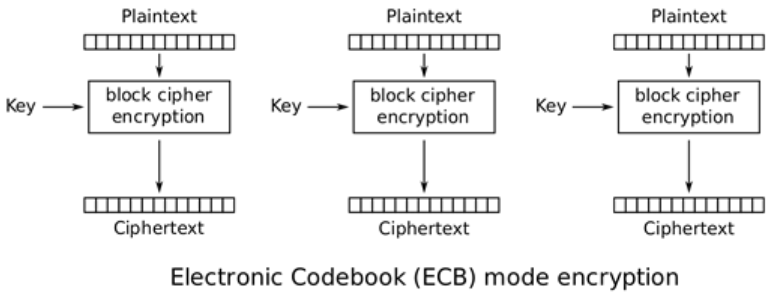
\includegraphics[width=0.9\textwidth]{ecb.png}
\end{figure}
Note that ECB mode is not IND-CPA secure because it's deterministic 

\subsection{CBC mode of operation}
We use an initialization vector (IV) to compute the first block's ciphertext given the encryption function $E(K, M)$
\begin{enumerate}
    \item $C_1 = E(K, M_1 \oplus IV)$
    \item $C_2 = E(K, M_2 \oplus C_1)$
    \item $C_3 = E(K, M_3 \oplus C_2)$
    \item $\vdots$
    \item $C_n = E(K, M_n \oplus C_{n-1})$
\end{enumerate}
\begin{figure}[H]
    \centering
    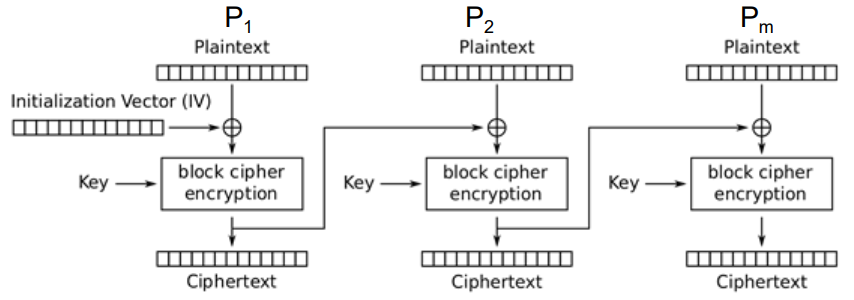
\includegraphics[width=0.9\textwidth]{cbc.png}
\end{figure}
\newpage
\noindent \textbf{CBC decryption:} Given $K, IV, C_1, C_2, \ldots, C_n$ we can compute $M_1, M_2, \ldots, M_n$ as follows:

\begin{enumerate}
    \item $D(K, C_1) \oplus IV = M_1$
    \item $D(K, C_2) \oplus C_1 = M_2$
    \item $D(K, C_3) \oplus C_2 = M_3$
    \item $\vdots$
    \item $D(K, C_n) \oplus C_{n-1} = M_n$
\end{enumerate}

\subsection{Padding}
Padding schemes:
\begin{itemize}
    \item We cannot padd with only 0's or only 1's because we cannot distinguish between padding and actual data
    \item We can pad with a 1 followed by 0's
\end{itemize}
PKCS \#7 padding:
\begin{itemize}
    \item If we need to pad $k$ bytes, we pad with $k$ bytes of value $k$
    \item For example, if we need to pad 3 bytes, we pad with 0x03 0x03 0x03
\end{itemize}

\noindent \textbf{CBC security:} AES-CBC is IND-CPA secure if IV is randomly chosen and never reused

\subsection{CBC: IV Reuse}
Assume we have these two 3-block messages
\begin{itemize}
    \item $M = P_1 || P_2 || P_3$
    \item $M' = P_1' || P_2' || P_4$
\end{itemize}
If $IV$ is reused for both messages in CBC mode the two first blocks for the second message can be revealed

\subsection{Counter Mode (CTR)}
\begin{itemize}
    \item \textbf{Encryption:} $E(K, M) = P_i \oplus E(K, Nonce_i) = C_i$
    \begin{itemize}
        \item $C = C_1 || C_2 || \ldots || C_n$
    \end{itemize} 
    \item \textbf{Decryption:} $D(K, C_i) = C_i \oplus E(K, Nonce_i) = P_i$
    \begin{itemize}
        \item $P = P_1 || P_2 || \ldots || P_n$
    \end{itemize}
\end{itemize} 
Nonce is a unique value for each block e.g. a counter and it should never be reused
\begin{figure}[H]
    \centering
    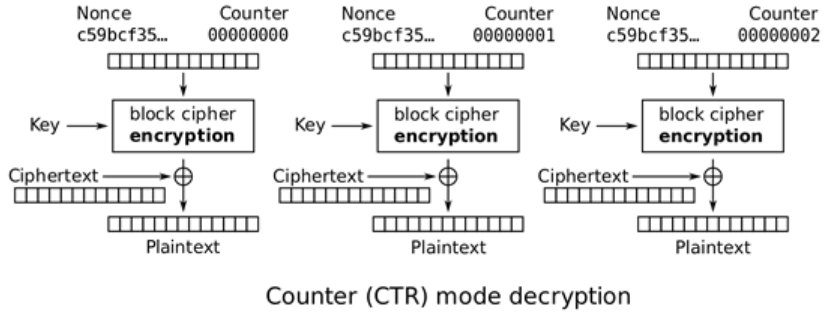
\includegraphics[width=0.5\textwidth]{ctrdec.png}\hfill
    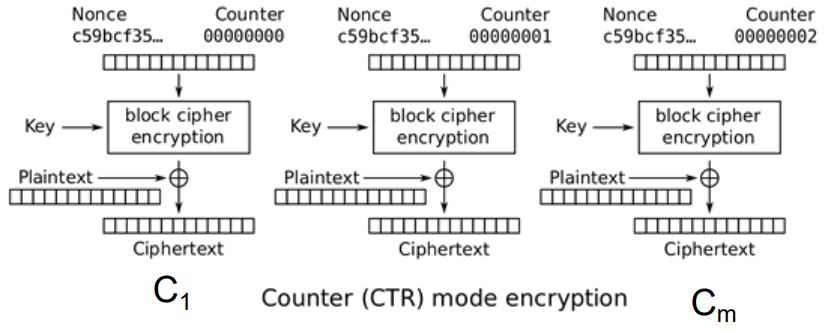
\includegraphics[width=0.5\textwidth]{ctrenc.png}
\end{figure}
\begin{itemize}
    \item Both encryption and decryption can be done in parallel because each block is independent of the others
    \item Padding is not needed because we can just XOR the last block with the first $k$ bits of the keystream
\end{itemize}

\subsection{CTR mode security}
\begin{itemize}
    \item AES-CTR is IND-CPA secure if nonce is never reused
    \item If nonce is reused it would be equivalent to key reuse in a one-time pad which is not secure
\end{itemize}

\subsection{CTR vs CBC}
\begin{itemize}
    \item Both AES-CBC and AES-CTR are IND-CPA secure are equally secure if used correctly 
    \item AES-CTR is more efficient because of parallelization 
    \item AES-CBC is safer because only partial information is revealed if IV is reused
    \item AES-CTR reveals everything if nonce is reused once
\end{itemize}
\subsection{Block cipher: integrity and authenticity}
\textbf{CTR:}
\begin{itemize}
    \item Mallory can tamper with the ciphertext and the decrypted plaintext will be different
    \item The receiver will not know that the message has been tampered with
\end{itemize}

\noindent \textbf{CBC}:
\begin{itemize}
    \item If Mallory tampers with the ciphertext the decrypted plaintext will be jibberish
    \item The receiver will know that the message has been tampered with
\end{itemize}

\subsection{Public key cryptography}
A scheme where each person has two keys:
\begin{itemize}
    \item \textbf{Public key:} Known to everyone
    \item \textbf{Private key:} Only known to the owner
    \item Uses number theory to create one way functions 
    \item Alice and Bob no longer need to share a secret key
    \item \textbf{Drawback:} Public key cryptography is much slower than symmetric key cryptography
\end{itemize}

\subsection{Diffie-Hellman Key Exchange}
%% Contninue Lecture 5 page 53












\end{document}§